\begin{figure}[t]
\centering
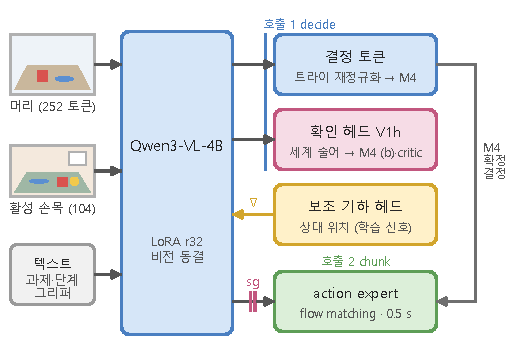
\includegraphics[width=\linewidth]{figures/model.pdf}
\caption{\textbf{조이스틱 VLA.} 머리 카메라와 활성 팔 손목 카메라를 원본 해상도 다중 이미지로 넣고, 과제 문장·구간 의도 줄·그리퍼 상태·움직임 줄을 붙인다. 결정 스텝마다 두 번 부른다. \textbf{decide}: 한 번의 순전파로 결정 토큰의 보기 확률(\cref{eq:trie})과 확인 헤드 V1h의 세계 쪽 술어를 낸다. 보조 기하 헤드는 시뮬 특권 상태의 상대 위치를 예측하는 학습 신호이며 실행 때는 쓰지 않는다. \textbf{chunk}: 행동 전문가가 기울기 차단(KI) 뒤의 문맥 은닉 상태를 읽고, M4가 확정한 결정을 조건으로 0.5\,s 청크를 낸다. 전문가가 결정을 따르게 하는 것은 먼 구간 반사실 분기 학습이 맡는다(\cref{sec:vla}). 영상 탑은 얼리고, 헤드 크기와 손실 가중치는 \tentative{가정값}이다.}
\label{fig:model}
\end{figure}
